\section{Results}
Figure~\ref{fig:abp-filters} indicates the different types of filters  present in adblock.
The horizontal axis lists the domains associated with the webpages and the vertical axis lists the type of filter fired. The size of the circle corresponds to  the proportion of elements in that domain that are of a particular element type as indicated in the corresponding vertical axis. Looking at  particular domain from top to bottom shows the composition of various elements in the web pages belonging to that domain. In most of the cases  SCRIPT,IMAGE and SUBDOCUMENT can be seen as the dominating elements. These are the elements which the Adblock plus browser addon counts as an advertisement as a part of its statistics gathering.
\begin{figure}[h]
	\centering
	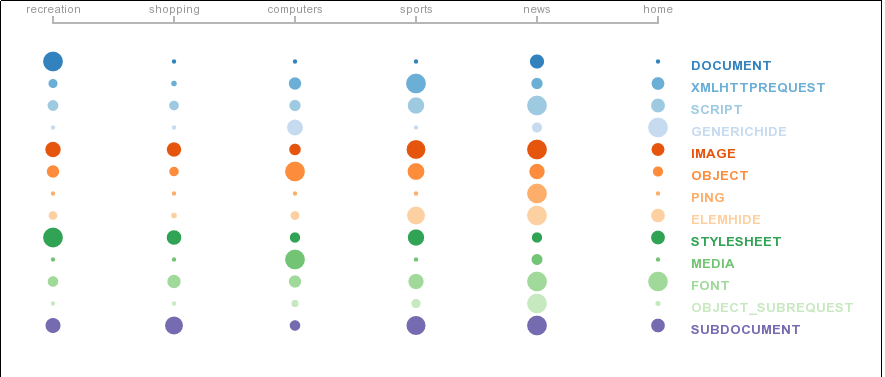
\epsfig{file=figures/abp_filters.png, width=0.50\textwidth}
	\vspace*{-0.5cm}
	\caption{\textbf{Filter Types in Adblock Plus}}
	\label{fig:abp-filters}
	\vspace*{-0.5cm}
\end{figure}

Figure~\ref{fig:growth}, indicates the growth of whitelist since 2012. The aacceptable ads program had initially 132 filters in it. Over the years the whitelist has grown enormously in  size.  Over 3600 filters were added  between 2012 to 2013 and the list has been growing. As of March 2016, the total number of  filters in the whitelist is 6570.
\begin{figure}[p]
	\centering
	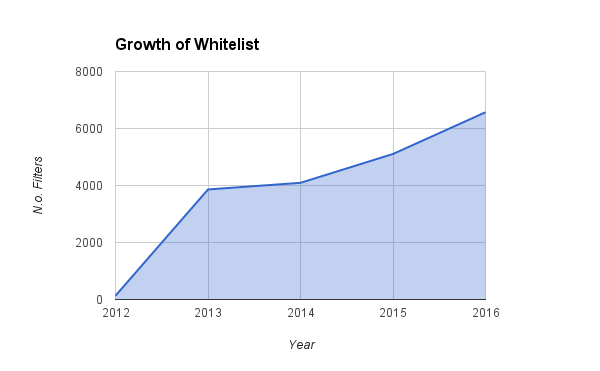
\epsfig{file=figures/growth.png, width=0.50\textwidth}
	\vspace*{-0.5cm}
	\caption{\textbf{Growth of Whitelist.}}
	\label{fig:growth}
	\vspace*{-0.5cm}
\end{figure}

Unsurprisingly, one can see an increasing trend in the number of ads allowed by adblock plus.
Figure~\ref{fig:ads-allowed}, shows the trend in the ads allowed over the years.
\begin{figure}[p]
	\centering
	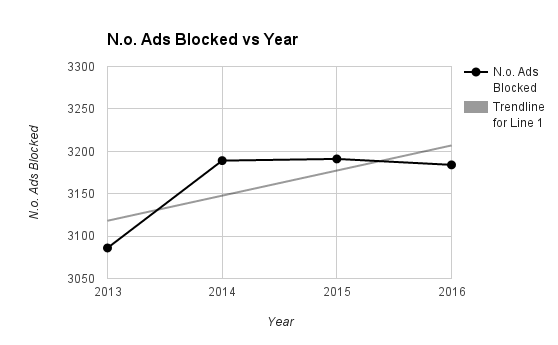
\epsfig{file=figures/alexa_ads.png, width=0.50\textwidth}
	\vspace*{-0.5cm}
	\caption{\textbf{Number of Ads allowed in the Alexa top 200.}}
	\label{fig:ads-allowed}
	\vspace*{-0.5cm}
\end{figure}

Fig~\ref{fig:block-allow} shows the difference between the number of  elements  blocked  versus the number of elements allowed for three different  combuinations of the filters.
It can be seen that the list with only the element hiding filter does poorly in blocking the  elements as it does not have the capabilities of blocking URLS.
As expected the easylist+whitelist combination allows more ads there by allowing more elements.
\begin{figure}
	\centering
	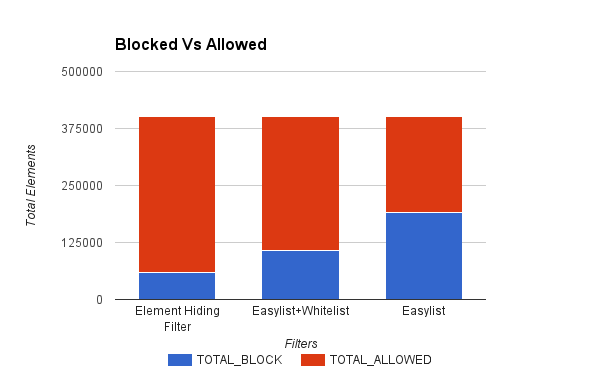
\epsfig{file=figures/exp_comparison.png, width=0.50\textwidth}
	\vspace*{-0.5cm}
	\caption{\textbf{Blocked vs Allowed for filter combinations}}
	\label{fig:block-allow}
	\vspace*{-0.5cm}
\end{figure}

To demonstrate how AdBlock Plus can be too restrictive in the sense of blocking elements that are not ads we set up a simple page that handles a GET request with 'admid' as a query parameter. AdBlock Plus has 'admid' in its blacklist and hence doesn't even allow the call to pass through. This is a big limitation to the pattern-matching approach to blacklisting, in that legitimate content of publishers would get to be not displayed.

AdBlock Plus is not capable of finding out all elements that are ads, as well. As explained earlier, we used the bit.ly redirection URL within the page instead of the actual URL. As in the figure, the AdBlock Plus has an element hiding filter that blocks the image. It doesn't block the image underneath it, even though it refers to the same site - this can be seen in the figure (x) where no ad-blocking is applied.

However, this does not work with the URL blocking filter. This is because bit.ly being a URL redirection filter, it returns the original URL which is then blocked by the URL filter. In this case, we developed a proxy site that essentially renders it as a call to a different URL. In the future work section we discuss other possible approaches as well.


